\documentclass[conference]{IEEEtran}
\IEEEoverridecommandlockouts
% The preceding line is only needed to identify funding in the first footnote. If that is unneeded, please comment it out.
\usepackage{cite}
\usepackage{amsmath,amssymb,amsfonts}
\usepackage{algorithmic}
\usepackage{graphicx}
\usepackage{textcomp}
\usepackage{xcolor}
\usepackage{url}
\usepackage{listings}
\usepackage{caption}

\captionsetup[lstlisting]{position=bottom}
\def\BibTeX{{\rm B\kern-.05em{\sc i\kern-.025em b}\kern-.08em
    T\kern-.1667em\lower.7ex\hbox{E}\kern-.125emX}}

% Suppress overfull/underfull \hbox warnings
\hfuzz=10pt        % allows overfull hboxes up to 10pt without warning
\hbadness=10000    % suppresses underfull hbox warnings
\vbadness=10000    % suppresses underfull vbox warnings

\begin{document}

\title{Serverless Dataflows}
% {\footnotesize \textsuperscript{*}Note: Sub-titles are not captured in Xplore and
%should not be used}
%\thanks{Identify applicable funding agency here. If none, delete this.}

% \author{\IEEEauthorblockN{1\textsuperscript{st} Diogo Jesus}
\author{\IEEEauthorblockN{Diogo Jesus}
% \IEEEauthorblockA{\textit{dept. name of organisation (of Aff.)} \\
\IEEEauthorblockA{
\textit{Instituto Superior Tecnico (IST), INESC-ID Lisboa}\\
Lisbon, Portugal \\
diogofjesus@inesc-id.pt}}
\maketitle

\begin{abstract}
Serverless computing has become a suitable cloud paradigm for many applications, prized for its operational ease, automatic scalability, and fine-grained pay-per-use pricing model. However, executing workflows, which are compositions of multiple tasks, in Function-as-a-Service (FaaS) environments remains inefficient. This inefficiency stems from the stateless nature of functions, and a heavy reliance on external services for intermediate data transfers and inter-function communication.

In this document, we introduce a decentralized DAG engine that leverages historical metadata to plan and influence task scheduling. Our solution encompasses metadata management, static workflow planning, and a worker-level scheduling strategy designed to drive workflow execution with minimal synchronization. We compare our system against WUKONG, another decentralized serverless DAG engine, and Dask Distributed, a more traditional cluster-based DAG engine. Our evaluation demonstrates that utilizing historical information significantly improves performance and reduces resource utilization for workflows running on serverless platforms.
\end{abstract}

\begin{IEEEkeywords}
Cloud Computing, Serverless, FaaS, Serverless Workflows, DAG, Metadata, Workflow Prediction
\end{IEEEkeywords}

\section{Introduction}
\label{s:introduction}

Function-as-a-Service (FaaS) represents a serverless cloud computing paradigm that simplifies application deployment by abstracting away infrastructure management. It provides automatic, elastic scalability—potentially without limit—along with a fine-grained, pay-per-use pricing model. This has led to its widespread adoption for event-driven systems, microservices, and web services on platforms like AWS Lambda\footnote{\label{fn:aws-lambda}https://aws.amazon.com/pt/lambda/}, Azure Functions\footnote{\label{fn:azure-funcs}https://azure.microsoft.com/en-us/products/functions}, and Google Cloud Functions\footnote{\label{fn:google-cloud-functions}https://cloud.google.com/functions}. These applications typically benefit the most from FaaS because they are lightweight, stateless, and characterized by highly variable or unpredictable workloads, allowing them to leverage serverless platforms' on-demand scalability and cost-efficiency.

This paradigm is also increasingly used to execute complex scientific and data processing workflows, such as the Cybershake~\cite{cybershake_workflow} seismic hazard analysis or Montage~\cite{montage_astronomy}, an astronomy image mosaicking workflow. These applications are structured as workflows—formally represented as Directed Acyclic Graphs (DAGs) of interdependent tasks. However, efficiently executing these complex workflows on serverless platforms remains a significant challenge. 

Despite their advantages, serverless platforms present several limitations that complicate the execution of complex workflows. Since these platforms allow scaling down to zero resources to save costs, they can also introduce unpredictable latency, known as \textit{cold starts}~\cite{cold_starts_surey}, particularly for short-lived functions, affecting overall workflow performance. The lack of \textit{direct inter-function communication}~\cite{serverless_computing_drawbacks_survey_rw1} means that tasks often have to rely on external services, such as message brokers or databases to exchange intermediate data, which can increase overhead and reduce efficiency. Interoperability between platforms is further limited by the use of platform-specific workflow definition languages, which restricts the portability of workflows across different serverless environments. Additionally, while statelessness simplifies scaling and management, it can introduce overhead and complexity for applications that require continuity or coordination across multiple function invocations. Finally, developers have limited control over the underlying infrastructure, restricting the ability to optimize resource usage or tune performance for specific workloads.

Several solutions have emerged to address the limitations of serverless platforms. Stateful functions (e.g., AWS Step Functions\footnote{\label{fn:aws-step-functions}https://aws.amazon.com/pt/step-functions/}, Azure Durable Functions\footnote{\label{fn:azure-durable-functions}https://learn.microsoft.com/en-us/azure/azure-functions/durable/durable-functions-overview?tabs=in-process\%2Cnodejs-v3\%2Cv1-model\&pivots=csharp}, and Google Cloud Workflows\footnote{\label{fn:google-cloud-workflows}https://cloud.google.com/workflows}) expand the range of applications that can run on serverless platforms by maintaining state across multiple function invocations, coordinating complex workflows, and providing built-in fault tolerance. Other approaches tackle limitations at the runtime level, proposing extensions to FaaS platforms (e.g., Faa\$T~\cite{faast_caching}, Palette~\cite{palette_load_balancing}, Lambdata~\cite{lambdata_intents}) or entirely new serverless architectures (e.g., Apache OpenWhisk~\cite{open_whisk}). Finally, some workflow-focused solutions (e.g., WUKONG~\cite{wukong_2}, Unum~\cite{unum_decentralized_orchestrator}, DEWEv3~\cite{dewe_v3}) employ scheduling strategies and workflow-level optimizations to enhance efficiency, primarily by improving data locality to bring computation closer to the data and minimize reliance on external services.

These workflow-focused approaches, however, often use uniform resources for workers and rely on “one-step scheduling,” making decisions based solely on the immediate workflow stage without considering the broader context or the downstream effects of their decisions. This combination of homogeneous worker configurations and limited scheduling foresight can lead to inefficient use of resources when tasks have diverse computational or memory requirements. Furthermore, the heuristic-based approaches used by other solutions can be inefficient in certain scenarios, as they lack mechanisms to adapt worker resource allocations to the specific needs of individual tasks. Moreover, we found no prior work that leverages metadata or historical metrics to inform scheduling decisions across an entire serverless workflow.  

This limitation motivates the central research question of this work: if we have knowledge of the computation steps, collect sufficient metrics on their behavior, and understand how they are composed to form the full workflow, can we leverage this information to make smarter scheduling decisions that minimize makespan and maximize resource efficiency in a FaaS environment?  

To answer this research question, we propose a decentralized serverless workflow execution engine that leverages historical metadata from previous workflow runs to generate informed task allocation plans, which are then executed by FaaS workers in a choreographed manner, without needing a central scheduler. By relying on such planning, our approach aims to minimize the usage of external cloud storage services, which are often employed by similar solutions for intermediate data exchange and synchronization, while also avoiding the inefficiencies of homogeneous worker resource allocations.

The main contributions of this work are as follows:
\begin{itemize}
    \item Analysis of the serverless workflow orchestration research landscape;
    \item Propose a decentralized serverless workflow execution engine that overcomes the "one-step scheduling" and uniform-resource limitations of existing workflow-focused solutions by leveraging historical metadata to generate informed execution plans;
    \item Demonstrate how incorporating historical execution data can improve task allocation, reduce reliance on external cloud storage services, and enhance overall workflow efficiency on FaaS platforms.
\end{itemize}


% ------------------------------------------------ %

\section{Architecture}
\label{s:architecture}

While current serverless platforms excel at embarrassingly parallel jobs with short-duration tasks, they present challenges for workflows involving significant data exchange between tasks due to their architectural limitations, which do not allow inter-function communication and control over where each function is executed. In the future, however, serverless platforms are expected to improve, eventually overcoming these limitations and becoming a viable, user-friendly and cost-effective alternative to IaaS for a wide range of workflows.

As we have stated, most existing serverless schedulers employ an approach where decisions are made based solely on the immediate workflow stage without considering the global implications. We hereby propose a novel \textit{decentralized serverless workflow execution engine} that leverages historical metadata from previous workflow runs to make fast predictions and create workflow plans before they execute. Such plans include information about where to execute each task (locality), the worker resource configuration to use (how much vCPUs and Memory) and optimizations. At run-time, the workers will execute the plan and apply the specified optimizations. It was written in \textit{Python}, a language known for its simplicity and popularity among data scientists.

\subsection{Workflow Definition Language}
\label{ss:workflow_definition_language}

We will now present our DAG-based workflow engine that transforms ordinary Python functions into parallelizable tasks, automatically managing dependencies and execution through an intuitive decorator-based API. It is inspired by WUKONG, Dask and Airflow's way of expressing workflows: the user can create workflows by composing individual Python functions, as shown in Listing \ref{lst:dag_lang_example}. In this example, we define two tasks, \texttt{task\_a} and \texttt{task\_b}, and then compose them into a DAG by passing their results as arguments to the next task. The resulting workflow structure is illustrated in Figure \ref{fig:dag_lang_example}.

\begin{figure}[h]
\centering
\begin{lstlisting}[language=Python, basicstyle=\ttfamily\footnotesize, columns=fullflexible, breaklines=true]
# 1) Task definition
@DAGTask
def task_a(a: int) -> int:
    # ... user code logic ...
    return a + 1

@DAGTask(forced_optimizations=[PreLoadOptimization()])
def task_b(*args: int) -> int:
    # ... user code logic ...
    return sum(args)

# 2) Task composition (DAG/Workflow)
a1 = task_a(10)
a2 = task_a(a1)
a3 = task_a(a1)
b1 = task_b(a2, a3)
a4 = task_a(b1)
\end{lstlisting}
\caption{DAG definition example}
\label{lst:dag_lang_example}
\end{figure}

\begin{figure}[h]
    \centering
    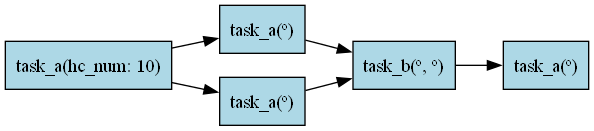
\includegraphics[width=\columnwidth]{figures/dag_lang_example.png}
    \caption{Simple DAG example}
    \label{fig:dag_lang_example}
\end{figure}

When \texttt{task\_a(10)} is invoked, it doesn't actually run the user code. It instead creates a representation of the task, which can be passed as argument to other tasks. The workflow planning and execution only happens once \texttt{.compute()} is called on the last/sink task (\texttt{a4}), as shown in Listing~\ref{lst:setup_and_launch_workflow_execution}. When \texttt{compute()} is called, we can create a representation of the entire workflow structure by backtracking the task dependencies.

\begin{figure}[h]
\centering
\begin{lstlisting}[language=Python, basicstyle=\ttfamily\footnotesize, columns=fullflexible, breaklines=true]
result = a4.compute(
    dag_name="simpledag", 
    config=Worker.Config(
        faas_gateway_address=...,
        intermediate_storage_config=(ip, port, password),
        metrics_storage_config=(ip, port, password),
        planner_config=UniformPlanner.Config(
            sla=sla,
            worker_resource_configuration=TaskWorkerResourceConfiguration(cpus=3, memory_mb=512),
            optimizations=[PreLoadOptimization, TaskDupOptimization]
        )
    )
)
\end{lstlisting}
\caption{Setting up and launching workflow execution}
\label{lst:setup_and_launch_workflow_execution}
\end{figure}

One limitation of this DAG definition language is that it doesn't support "dynamic fan-outs" (e.g., creating a variable number of tasks depending on the result of another task) on a single workflow. This is a powerful and expressive feature, but that is seldom supported in other DAG definition languages (e.g., Dask, WUKONG, Unum, Oozie~\cite{apache_oozie} do not support it). These languages require the user to split the workflow into multiple workflows, one for each \textit{dynamic fan-out}: one workflow runs up to the task that generates a list of results, while a second workflow starts with a number of tasks that depends on the size or contents of that list. 

Apache AirFlow~\footnote{https://airflow.apache.org/docs/apache-airflow/stable/authoring-and-scheduling/dynamic-task-mapping.html} supports this feature through an extension to their DAG language, allowing a variable number of tasks to be created at run-time depending on the number of results produced by a previous task. Implementing similar functionality is possible, but it would reduce the accuracy of predictions. This is because we would also need to predict the expected fan-out size, and any errors in that prediction could amplify inaccuracies in the predictions for the rest of the workflow.

We will now present the architecture, highlighting the core layers of our solution.

\subsection{Architecture Overview}

The overall architecture and logical flow of our decentralized serverless workflow execution engine is organized into 3 high-level layers. Figure~\ref{fig:solution_architecture} provides an overview of this architecture. The upper part represents the components that run on the user's machine, while the lower part represents the components that run outside the user's machine. 

The user writes its workflows in Python (demonstrated in Section \ref{ss:workflow_definition_language}). First, a planning algorithm, chosen by the user, will run locally to generate a static workflow plan. This plan defines a task-to-worker mapping and other task-level optimization hints for FaaS workers. Once the plan is done, the client launches the initial workers for the root tasks, kicking off workflow execution. The user program then waits for a storage notification indicating workflow completion and then retrieves the final result from storage.

The following sections should provide a deeper understanding of each layer as well as how the user interacts with the system.

\begin{figure}[h]
  \centering
  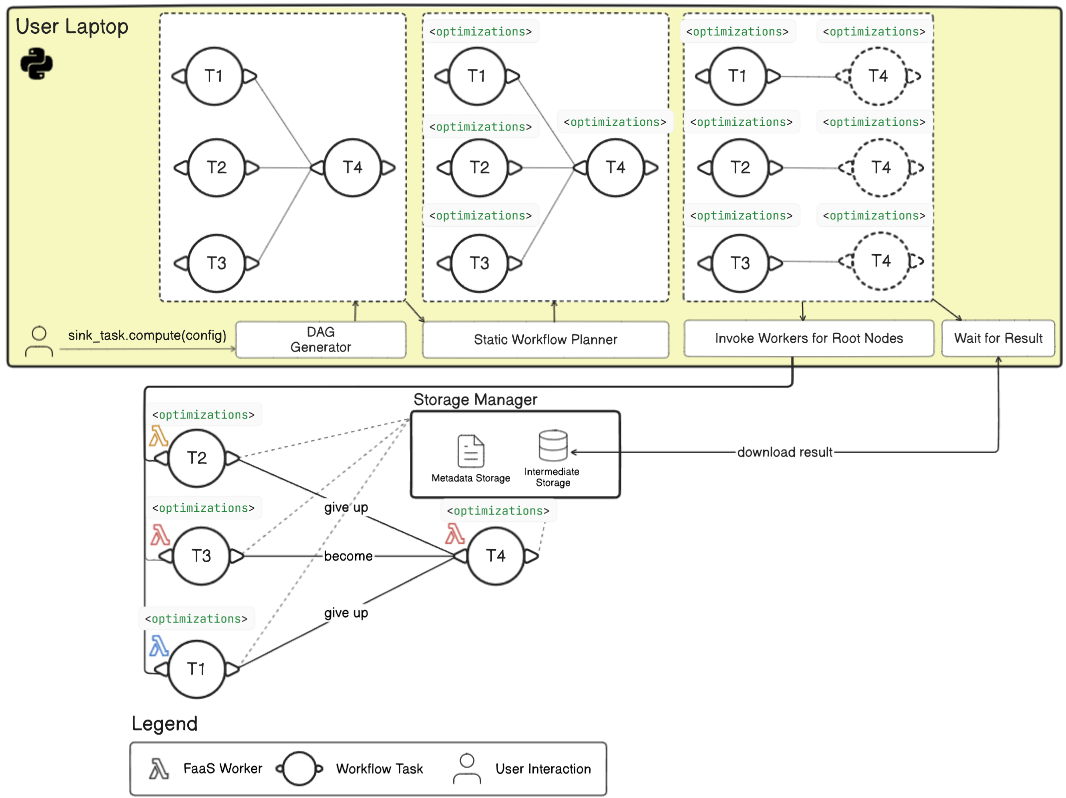
\includegraphics[width=\columnwidth]{figures/solution_distributedarchintegrated.png}
  \caption{Solution Architecture}
  \label{fig:solution_architecture}
\end{figure}

\begin{enumerate}
    \item \textbf{Metadata Management}: Responsible for collecting and storing task metadata from previous executions. It also uses this metadata to provide predictions regarding task execution times, data transfer times, task output sizes, and worker startup times;
    \item \textbf{Static Workflow Planning}: Receives the entire workflow, represented as a Directed Acyclic Graph (DAG), and a "planner" (an algorithm chosen by the user). This planner will use the predictions provided by Metadata Management to create a static plan/schedule to be followed by the workers;
    \item \textbf{Scheduling}: This component is integrated into the workers, and it is responsible for executing the plan generated by the Static Workflow Planning layer, applying optimizations and delegating tasks as needed.
\end{enumerate}

There are 3 distinct computational entities involved in this system:

\begin{itemize}
    \item \textbf{User Computer}: Responsible for creating workflow plans, submitting them (triggering workflow execution), and receiving its results. The planning phase also happens on this computer, right before a workflow is submitted for execution;
    \item \textbf{Workers}: These are the FaaS workers (often running in containerized environments), that execute one or more tasks. The decentralization of our solution is due to the fact that these workers are responsible for scheduling of subsequent tasks, delegating tasks and launching new workers when needed without requiring a central scheduler. Lastly, they are also responsible for collecting and uploading metadata;
    \item \textbf{Storage}: Consists of an \textit{Intermediate Storage} for intermediate outputs which may be needed for subsequent tasks and a \textit{Metadata Storage} for information crucial to workflow execution (e.g., notifications about task readiness and completion).
\end{itemize}

Next, we will explain how the user defines and submits workflows for execution.

\subsection{Metadata Management}
\label{ss:metadata_management}
The goal of the \textbf{Metadata Management} layer is to provide the most accurate task-wise predictions to help the planner algorithm chosen by the user to make better decisions. To achieve this, while the workflow is running we collect metrics about each task's execution. These metrics are stored in \textit{Metadata Storage}: task execution time, data transfer size and time, task input and output sizes, and worker startup time. 

Storing these metrics enables us to provide a prediction API, shown in Listing~\ref{lst:task_predictions_api}. To improve accuracy, metrics are kept separate for each workflow. As a result, even if two workflows use the same function or task code, their metrics are stored independently. This design choice reflects our assumption that different workflows may follow different execution patterns. To avoid introducing runtime overhead, metrics are batched and uploaded when the worker shuts down.

The prediction methods take an additional parameter, \texttt{SLA} (Service-level Agreement), which is specified by the user and influences the selection of prediction samples. For example, \texttt{SLA="median"} will use the median of the historical samples, whereas \texttt{SLA=Percentile(80)} will return a more conservative estimate. By allowing the user to control this parameter, the API can provide predictions that are tailored to different performance requirements.

\begin{figure}[h]
\centering
\begin{lstlisting}[basicstyle=\ttfamily\footnotesize, columns=fullflexible, breaklines=true]
class PredictionsProvider:
  def predict_output_size(function_name, input_size, sla) -> int

  def predict_worker_startup_time(resource_config, state: 'cold' | 'warm', sla) -> float

  def predict_data_transfer_time(
        type: 'upload' | 'download',
        data_size_bytes,
        resource_config,
        sla,
        scaling_exponent
    ) -> float

  def predict_execution_time(
        task_name,
        input_size,
        resource_config,
        sla: SLA,
        size_scaling_factor
    ) -> float
\end{lstlisting}
\caption{Task Predictions API}
\label{lst:task_predictions_api}
\end{figure}

In addition, metrics such as worker startup time, data transfer time, and task execution time are tied to the specific worker resource configuration. To account for this, our prediction method follows two paths. If we have enough historical samples for the same resource configuration, we use only those. Otherwise, when there are not enough samples with the same resource configuration, we fall back to a normalization strategy: we adjust samples from other memory configurations to a baseline, use those to estimate execution time, and then rescale the result back to the target configuration. 

After filtering samples we use an algorithm that selects a limited number of the most relevant samples for each prediction. This algorithm works by gradually widening a tolerance window around the reference value until it finds enough nearby samples. Within each window, it balances samples that are smaller, larger, or exactly equal to the reference, giving preference to the closest ones. If there still aren't enough candidates, it falls back to simply picking the nearest available samples overall. This way, the algorithm adapts to the data while keeping the selection both relevant and limited in size.

\subsection{Static Workflow Planning}
This layer executes on the user side, and it receives the workflow representation and a workflow planning algorithm chosen by the user (as shown in Listing \ref{lst:setup_and_launch_workflow_execution}). Its job is to execute the planning algorithm, providing it access to the predictions exposed by the Metadata Management layer (Section \ref{ss:metadata_management}).

Planners can run \textit{workflow simulations} based on the predictions, allowing them to experiment with different resource configurations for different tasks and different task co-location strategies. Additionally, they can apply different user-selected optimizations. The accuracy of these simulations depends on the accuracy of the predictions exposed by the \textit{Predictions API}.

For each task, the planner assigns both a \texttt{worker\_id} and a resource configuration (vCPUs and memory). The \texttt{worker\_id} specifies the worker instance that must execute the task—analogous to the “colors” in Palette Load Balancing~\cite{palette_load_balancing}, but in our case this assignment is mandatory rather than advisory, giving strict control over execution locality. Two tasks assigned the same \texttt{worker\_id} should be executed on the same worker instance. If \texttt{worker\_id} is not specified, workers will, at run-time, have to decide whether to execute or delegate those tasks, similar to WUKONG's ~\cite{wukong_2} scheduling. We refer to these workers as \textit{"flexible workers"}.

Users can select from three provided planners or implement their own planner by implementing an interface. All planners have access to the predictions API as well as the workflow simulation. The planners the user can choose from are the following:

\begin{enumerate}
    \item \textbf{WUKONG}: All tasks will use the same worker configuration (specified by the user) and won't be assigned a \texttt{worker\_id}, meaning they will be executed by \textit{"flexible workers"}. This is a more dynamic scheduling approach where tasks aren't tied to specific workers that try to reproduce WUKONG's scheduling behavior;
    \item \textbf{Uniform}: Tasks share a common worker configuration specified by the user, with each task assigned a \texttt{worker\_id} to allow for co-location of tasks.
    \item \textbf{Non-Uniform}: Tasks can use different worker configurations (list of available resources is specified by the user). Each task is assigned a \texttt{worker\_id}. This algorithm starts by assigning the best available resources to all tasks. Then it runs a resource downgrading algorithm that attempts to downgrade resources of workers \textit{outside the critical path} as much as possible without introducing a new critical path.
\end{enumerate}

Both the \textbf{Uniform} and \textbf{Non-Uniform} planners follow a two-phase approach for task allocation: resource configuration assignment followed by worker ID assignment. The planners differ in their resource allocation strategies. The \textbf{Uniform planner} applies a single, user-specified CPU and memory configuration to all tasks, while the \textbf{Non-Uniform planner} selects the most powerful configuration from the user-specified options for each task. After resource configuration, both planners employ the algorithm detailed in Listing \ref{lst:worker_id_assignment} for worker ID assignment. This algorithm implements an intelligent clustering strategy with two primary objectives: launch as few new workers as possible while trying not to overload workers; and minimizing network data transfers by co-locating tasks whose outputs are expected to be larger. This clustering approach provides an additional benefit of reducing fan-in operation costs.

After this, the \textbf{Non-Uniform} planner runs an additional algorithm, shown in Listing \ref{lst:resource_downgrading_algorithm}, that attempts to downgrade resources of workers \textit{outside the critical path} as much as possible without introducing a new critical path, by iteratively simulating the effect of downgrading resources of workers \textit{outside the critical path} with different configurations.

With the information they have access to, planners can estimate whether it is worthwhile to offload a task to a more powerful worker. This involves weighing the overhead of uploading the input data, waiting for the worker to be provisioned, and then executing the task, against the alternative of simply executing the task on the current, less powerful worker.

Aside from their \texttt{worker\_id} and resource assignments, planners can also apply different \textbf{optimizations} to further improve the workflow execution. The optimizations to be used are selected by the user, as shown in Listing \ref{lst:setup_and_launch_workflow_execution}. Similarly to planners, we provide three optimizations: \textbf{pre-warm}, \textbf{pre-load} and \textbf{task-dup}, but it is also possible to create new optimizations and define how workers should react to them. Now, we will describe the three base optimizations and how they are assigned to tasks:

\begin{enumerate}
\item\textbf{pre-warm}(worker\_config) [Pre-warming Workers]:
\begin{itemize}
  \item \textit{Interpretation}: Tasks/Nodes with this optimization should perform a special invocation to the FaaS gateway that forces it to launch a new worker with the specified resource configuration \texttt{worker\_config}. This can be used to warm up workers ahead of time and mask cold start latencies;
  \item \textit{Assignment Logic}: For the nodes whose workers are expected to have cold starts, find the "optimal" node to perform the pre-warming by searching for nodes/tasks whose activity timing falls within a window (goal: avoid the pre-warmed worker from going cold before needed, while also not being warm too late). The optimization will be added to the "optimal" node, which will be responsible for doing the special "empty invocation" to the FaaS gateway.
\end{itemize}

\item\textbf{pre-load} [Pre-Loading Dependencies]:
\begin{itemize}
  \item \textit{Interpretation}: Workers assigned to tasks or nodes with this optimization should begin downloading the task's dependencies as early as possible. This prevents scenarios where a worker must fetch all dependencies at once. The optimization is effective only if the worker is active before executing the task, allowing it to download dependencies in parallel with other ongoing tasks. This is implemented by having the worker receive completion notifications from the \textit{Metadata Storage} for all tasks upstream of the optimized task;
  \item \textit{Assignment Logic}: First, all tasks with more than a configurable threshold of dependencies/upstream tasks are assigned the optimization. Then, an iterative process is used to optimize the workflow along its critical path using this optimization. First, the algorithm identifies the critical path and assigns the optimization to eligible nodes on it. The critical path is then recalculated: if the total execution time increases, the optimization is removed; if the execution time decreases but the critical path changes, the algorithm restarts with the new path. This process repeats until no further improvements are possible, or the algorithm hits a fixed iteration limit.
\end{itemize}

\item\textbf{task-dup} [Task Duplication]:
\begin{itemize}
  \item \textit{Interpretation}: Tasks or nodes with this optimization can be executed by other workers if doing so helps unlock dependent tasks more quickly. The task could be "duplicated" by workers that depend on its output. It is a trade-off between performance and resource utilization, allowing potentially faster execution at the cost of using additional compute resources;
  \item \textit{Assignment Logic}: Assigned to all nodes whose execution time and input size do not exceed predefined thresholds. Whether duplication actually occurs is decided at run-time. The optimization targets fast tasks with small inputs, as these are inexpensive to duplicate in terms of both downloading dependencies and execution. This way, even if duplication turns out to be unnecessary, the impact on performance and resource usage remains minimal.
\end{itemize}
\end{enumerate}
Because planners may sometimes lack sufficient information to make optimal decisions about optimization assignments, it is important to not only allow the user to select optimizations at the workflow-level, but also allow them the flexibility to specify optimizations at the \textit{task-level}. An example of this feature is shown in Listing~\ref{lst:dag_lang_example}, where the user requests that \texttt{task\_b} attempt to use the \textit{pre-load} optimization.

Once these optimizations are assigned, workflow planning is complete, and workers can begin execution. Because planning occurs on the user's machine (i.e., the machine launching the workflow), it is responsible for initiating the workflow by starting the initial workers. From that point onward, workers dynamically invoke additional workers as needed, following a choreographed, decentralized execution model.

\begin{figure*}[h]
    \centering
    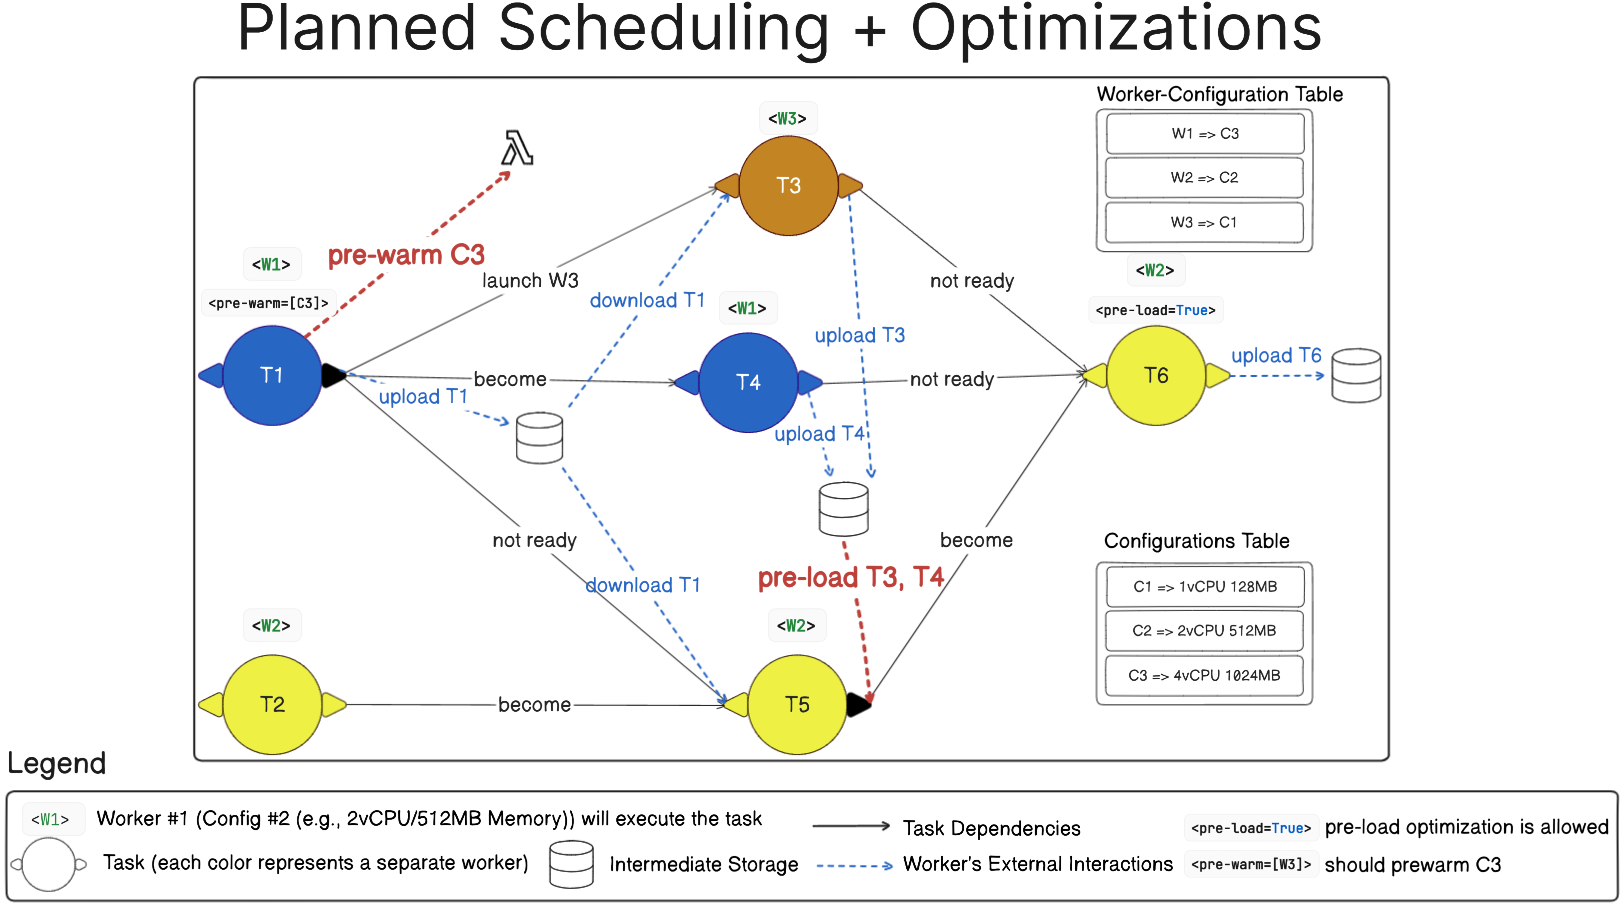
\includegraphics[width=\textwidth]{figures/solution_workflowinstanceexample.png}
    \caption{Planned Workflow Execution Example}
    \label{fig:planned_workflow_execution_example}
\end{figure*}

To illustrate this execution model, Figure~\ref{fig:planned_workflow_execution_example} provides a visual trace of how a planned workflow would be executed. The diagram depicts the workflow with the optimizations and \texttt{worker\_id} assignments for each task. The non-dashed arrows represent task dependencies, while the dashed arrows represent interactions with the \textit{Intermediate Storage} to either upload or download task data. We can see that task outputs are only uploaded to storage when there is at least one downstream task that depends on it and is assigned to another worker. 

It is also worth noting that the planner assigned \texttt{Task 6} to \texttt{Worker 2}. This decision might be due to \texttt{Worker 2} being more powerful than \texttt{Worker 1}, and because the output of \texttt{Task 5} is larger than that of \texttt{Tasks 4} and \texttt{5}. Therefore, even if the task were executed on a more powerful worker (such as \texttt{Worker 3}, which handled \texttt{Task 3}), the potential performance gain would not offset the additional time or resources required. This is an example of a planner deciding to co-locate \texttt{Tasks 5 and 6} on the same worker to reduce data movement.

Regarding \textbf{optimizations}, we can see \texttt{Task 1} \texttt{pre-warming} \texttt{Worker 3}, by making  a dummy invocation to the FaaS gateway, in an attempt to make it available before \texttt{Task 3} needs it. The \texttt{pre-load} optimization is used in \texttt{Task 5}, where the planner decided that \texttt{Worker 2} should start downloading the external dependencies for \texttt{Task 6} (\texttt{Task 3} and \texttt{Task 4}) as soon as they are available. This \texttt{pre-loading} can begin as soon as \texttt{Task 6}'s dependencies are ready in storage, potentially overlapping with \texttt{Task 2}'s execution instead of \texttt{Task 5}, as shown in the figure.


\subsection{Decentralized Scheduling}

Since our target execution platform is FaaS, the worker logic is implemented as a FaaS handler. Due to the decentralized nature of our solution, workers will be responsible for performing both task execution and scheduling in a choreographed manner. 

When invoked, a worker receives the \texttt{workflow\_id} and the \texttt{task\_ids} of the tasks it should execute first. Using this information, it retrieves the DAG structure and execution plan from \textit{Metadata Storage}. Rather than immediately executing the initial tasks, the worker first subscribes to \texttt{TASK\_READY} and \texttt{TASK\_COMPLETED} events for specific tasks. These events are essential both for enabling certain optimizations and for ensuring the worker follows the workflow plan correctly.

After that, the worker starts executing the initial tasks concurrently. The logic for executing tasks is the following:
\begin{enumerate}
    \item \textbf{Gathering Dependencies}: Check which dependencies are missing (not downloaded yet) and download them from storage;
    \item \textbf{Executing Task}: Execute the task. Tasks' code is stored in a serialized/pickled format (using cloudpickle\footnote{https://github.com/cloudpipe/cloudpickle}) and deserialized and executed by the workers. This enables the worker to remain generic, capable of receiving and executing arbitrary task code;
    \item \textbf{Handling Output}: This phase is responsible for evaluating whether it's necessary to upload the task's output to storage and emitting a \texttt{TASK\_COMPLETED} event;
    \item \textbf{Delegating Downstream Tasks}: For each downstream task, the worker performs an \texttt{atomic\_increment\_and\_get()} operation on a "dependency counter" (inspired by WUKONG~\cite{wukong_2}) stored in \textit{Metadata Storage}, which tracks how many dependencies of a task have been satisfied. When the counter indicates that all dependencies for a downstream task have been satisfied, the worker emits a \texttt{TASK\_READY} event for that task. The worker then consults the execution plan to determine how to proceed for each downstream task unlocked: if the unlocked task is assigned to another worker, a \texttt{TASK\_READY} event is emitted; if the unlocked task is assigned to the same worker and has no remaining dependencies, the worker immediately continues the cycle by executing it.
\end{enumerate}

To illustrate how workers handle downstream tasks, Figure~\ref{fig:choreographed_scheduling_example} presents an example of choreographed decentralized scheduling with three workers (A, B, and C) and seven tasks (T1-T7). In this example, once Task T1 completes on Worker B, the worker inspects the dependency counters for tasks T3, T4, and T5. It determines that T3 and T4 are ready to run, while T5 is still pending because Task T2 has not yet completed. Worker B then launches a new worker (C) to execute T3 and proceeds to execute T4 itself. Later, when T2 finishes on Worker A, all dependencies of T5 are satisfied, prompting Worker A to execute it directly.

\begin{figure}[h]
    \centering
    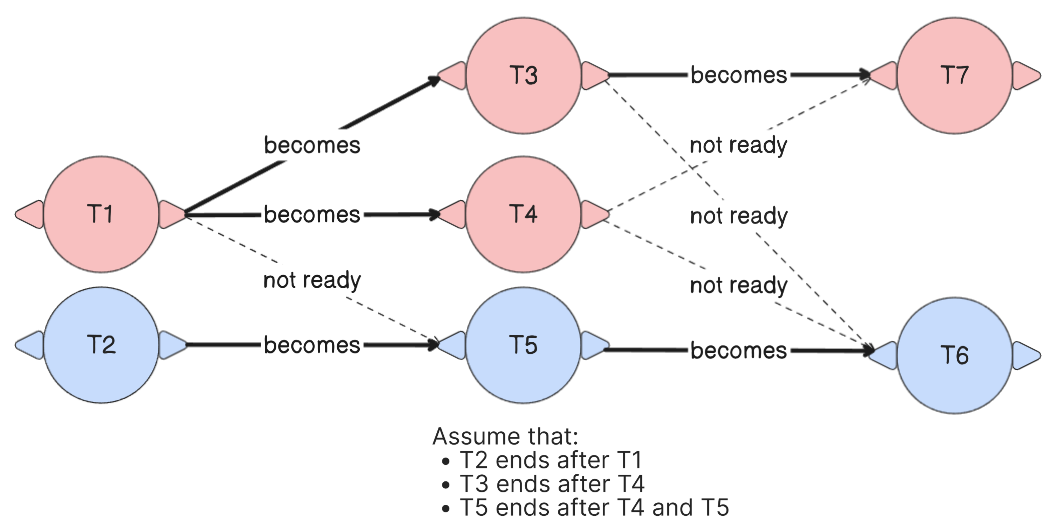
\includegraphics[width=0.5\textwidth]{figures/choreographed_execution_example.png}
    \caption{Choreographed Scheduling Example}
    \label{fig:choreographed_scheduling_example}
\end{figure}

A workflow is considered complete once the output of the final (sink) task is available in storage. The worker that uploads this final result is also responsible for cleaning up all intermediate results before shutting down. Meanwhile, after submitting the workflow, the user's machine subscribes to the \texttt{TASK\_COMPLETED} event for the sink task; upon receiving this notification, it retrieves the final result from \textit{Intermediate Storage}.

By delegating downstream tasks to workers, our approach eliminates the need for a central scheduler, a common component in many existing FaaS-based workflow engines. This decentralization increases flexibility and scalability, as workers can dynamically invoke additional workers as needed, following a choreographed decentralized execution model.

Having described the design and implementation of the system, we now turn to its evaluation. The next section presents the experimental setup, results, and analysis used to assess the strengths and weaknesses of our approach.

% ------------------------------------------------ %

\section{Evaluation and Analysis}

\subsection{Testing Environment}
%TODO: explain Docker simulating faas environment
\textbf{TODO: explain Docker simulating faas environment}
\subsection{Testing Configurations}
%TODO: worker resources, workflows, planners, SLAs
\textbf{TODO: worker resources, workflows, planners, SLAs}
\subsection{Results}
%TODO:
\subsection{Analysis}

% ------------------------------------------------ %


\section{Related Work}
\label{s:related_work}

This section highlights the most relevant related systems to our work, tracing the evolution from traditional cluster-based frameworks to modern cloud-native workflow orchestration platforms and serverless workflow engines. We highlight their key design principles, limitations, and the innovations that inspired our approach.

\subsection{Traditional Workflow Scheduling}
Traditionally, executing computation workflows has relied on distributed data processing frameworks designed to manage computation and data across clusters of machines. Frameworks such as Hadoop~\cite{apache_hadoop}, Apache Spark~\cite{apache_spark}, and Apache Flink~\cite{apache_flink} provide abstractions for parallel and distributed execution, enabling efficient coordination, scheduling, and data movement across clusters. A key programming model that influenced these systems is MapReduce~\cite{mapreduce}, which allows developers to process massive datasets by implementing simple \texttt{map} and \texttt{reduce} operations, with canonical example jobs like WordCount. Spark and Flink extend this model with in-memory processing and stream-oriented computation. More recently, Dask~\cite{dask_python} has emerged as a flexible Python-based framework that enables parallel and distributed execution of complex task graphs. Unlike traditional MapReduce-style frameworks, Dask supports a more generic programming model that goes beyond simple map and reduce operations, allowing execution of heterogeneous tasks across clusters while maintaining ease of integration with Python libraries. Dask is particularly well-suited for data science applications due to its seamless integration with NumPy, Pandas, and other libraries, and its ability to handle large-scale mathematical computations efficiently and in a distributed manner, through Dask Distributed~\cite{dask_python_distributed}.

Collectively, these frameworks rely on clusters of machines to distribute computation and manage data, providing scalability and parallelism for large-scale workflows. They offer several advantages, including control over the underlying system, easier to achieve better data locality, efficient use of dedicated resources, and the flexibility to fine-tune scheduling and execution policies. These features make them well-suited for complex, resource-intensive workloads where predictable performance is critical. However, the cluster-based approach also introduces overheads and has inherent limitations related to ease-of-use, deployment, resource provisioning, and slow resource scaling, which can limit performance and efficiency, particularly for dynamic and embarrassingly parallel workflows.

\subsection{Cloud-Native Workflow Scheduling}
Traditional cluster-based frameworks often require significant expertise to configure, deploy, and maintain. Cloud-native workflow solutions provide a higher-level, managed approach, enabling developers to orchestrate workflows without worrying as much about underlying infrastructure. These platforms simplify deployment, and automatically handle resource allocation, fault tolerance, and state management.

Prominent commercial serverless workflow platforms, also referred to as \textbf{stateful functions}, include AWS Step Functions~\textsuperscript{\ref{fn:aws-step-functions}}, Azure Durable Functions~\textsuperscript{\ref{fn:azure-durable-functions}}, and Google Cloud Workflows~\textsuperscript{\ref{fn:google-cloud-workflows}}. These solutions allow the user to create workflows by composing \textit{stateless} functions together. The platform is then responsible for the orchestration part, managing workflow state, intermediate results, and fault tolerance without requiring developers to implement state management themselves. These platforms typically employ \textit{checkpointing} techniques to persist workflow state, allowing the orchestrator or stateful function to pause while waiting for stages of the workflow to complete and then resume execution to trigger subsequent stages. Checkpointing also ensures that workflow execution can recover correctly after failures.

This orchestration and management capability is typically billed separately, reflecting both the convenience and reliability it provides and the additional resources required to maintain workflow state and fault tolerance. The main differences among these platforms lie in their execution model, workflow definition, and target use cases. Both AWS Step Functions and Google Cloud Workflows use JSON to represent workflow state machines, while Azure Durable Functions provides a more flexible programming model, where workflows are defined in code. One advantage of using such commercial services is that integration with other cloud services is easier, as they are tightly integrated with the AWS, Azure, and Google Cloud ecosystems.

In addition, there are also open-source workflow orchestration projects that run on general-purpose cloud or on-premises infrastructure, combatting vendor lock-in by providing better interoperability and flexibility. Apache Airflow~\cite{apache_airflow} is a widely used example, allowing workflows to easily be defined in Python code. Airflow has a rich ecosystem of pre-built integrations for databases, message queues, and major cloud services, simplifying the connection of workflows to diverse external services. It is mostly used for ETL ~\footnote{\label{fn:etl}https://pt.wikipedia.org/wiki/Extract,\_transform,\_load} processes, machine learning workflows, and batch data processing.

\subsection{FaaS Runtime Extensions}
While commercial and open-source workflow platforms simplify orchestration and state management, they generally operate on top of standard FaaS runtimes and cannot fully address the inefficiencies inherent in serverless platforms, such as cold starts, limited inter-function communication, and lack of data locality. To address these limitations, a significant body of research has focused on modifying the underlying FaaS runtime or proposing extensions that improve data locality and scheduling efficiency. Palette~\cite{palette_load_balancing}, Faa\$T~\cite{faast_caching}, and Lambdata~\cite{lambdata_intents} are three prominent examples of such extensions.

\subsubsection{Palette Load Balancing}
Palette Load Balancing improves data locality by introducing the concept of \textit{colors} as \textit{locality hints}. These colors are parameters attached to function invocations, allowing users to express which invocations should be co-located on the same worker. Palette then attempts to route invocations with the same color to the same instance, enabling subsequent invocations to access locally cached data rather than fetching it from remote storage. Colors are treated as \textit{hints}, so the system can ignore them if resource constraints require it. This approach improves cache hit ratios, reduces data transfer costs, gives enough flexibility to users or systems leveraging the runtime to define coloring policies with different strategies.

\subsubsection{Faa\$T}
Faa\$T provides a transparent, auto-scaling distributed cache for serverless functions. Each application has its own dedicated in-memory cache, called a \textit{cachelet}, which stores data accessed during function executions and makes it available for subsequent calls. Faa\$T's transparency is achieved by operating without requiring changes to application code, as it intercepts data requests and checks the cache before accessing remote storage. \textit{Cachelets} collaborate to form a distributed cache using consistent hashing, dynamically scaling up or down based on application workload.

\subsubsection{Lambdata}
Lambdata focuses on optimizing data locality by using \textit{user-provided data intents}. Developers explicitly annotate functions with \textit{get\_data} and \textit{put\_data} parameters, specifying which data objects the function will read or write. Lambdata then uses these annotations to make informed scheduling decisions such as co-locating functions that share data and leveraging local caches to minimize remote data transfers. This approach simplifies deployment and integration, as it does not require a distributed cache or complex runtime modifications, but relies on accurate intent declarations to achieve effective data reuse.

Together, these FaaS runtime extensions illustrate different strategies for improving data locality and execution efficiency in serverless environments.

\subsection{Serverless Workflow Scheduling Execution Engines}

Several frameworks have been designed to execute workflows efficiently on \textbf{unmodified} FaaS infrastructure, each offering distinct approaches to address the challenges of stateless, distributed computing. These solutions represent significant innovations in workflow orchestration, with varying trade-offs in terms of scalability, data locality, architectural complexity and ease-of-use and inspired our work. Here we will mention the most relevant workflow execution engines built to run on top of FaaS.

\subsubsection{DEWE v3}
DEWE v3~\cite{dewe_v3} introduces an innovative hybrid approach to serverless workflow orchestration that combines the best aspects of both serverless and serverful computing models. This hybrid workflow execution engine intelligently distributes tasks based on their characteristics: \textit{short tasks} are run on FaaS workers while \textit{longer tasks} run on virtual machines. The system employs a queue-based job distribution mechanism where jobs expected to complete within FaaS limits are published to a common job queue for serverless execution, while long-running jobs are directed to a separate queue for local, serverful execution on dedicated servers. Jobs that fail to execute on FaaS workers, for being longer than expected and exceeding execution limits imposed by the platform, are redirected to the serverful queue. This dual-execution model enables DEWE to accommodate workflows with diverse resource consumption patterns. This system proves particularly effective for scientific workflows, such as Montage~\cite{montage_astronomy}, where task durations and resource requirements vary significantly. However, this hybrid approach introduces specific trade-offs. Latency-sensitive workflows may be slowed by job queuing overhead. In addition, hybrid deployments often lead to resource underutilization, as serverful workers may sit idle when most tasks are executed on FaaS. Finally, the centralized workflow manager can become a scalability bottleneck when handling many short tasks.

\subsubsection{PyWren}
PyWren~\cite{pywren}, representing one of the pioneering pure serverless approaches, demonstrates the potential and limitations of leveraging unmodified serverless infrastructure for distributed computation. Built atop AWS Lambda, PyWren focuses on executing arbitrary Python functions as stateless serverless functions with minimal user management overhead, automatically handling function execution, dependencies, S3 bucket storage for serialized code and intermediate data. The system is ideal for embarrassingly parallel workloads, also known as \textit{"bag-of-tasks"} scenarios, with many independent, parallel tasks such as simple data transformations, scientific simulations, parallel model training, and large-scale media processing. While PyWren’s serverless orchestration model provides excellent scalability and removes the burden of infrastructure management, its simplicity limits its applicability. It is not well-suited for workflows with complex dependency structures or those that require sharing large intermediate results through object storage. Moreover, latency-sensitive applications are disadvantaged by function cold starts, since PyWren does not include mechanisms to mitigate their impact.

\subsubsection{Unum}
Unum~\cite{unum_decentralized_orchestrator} takes a radically different approach from the two previous solutions by decentralizing orchestration logic entirely, eliminating the need for a standalone orchestrator service. This application-level serverless workflow orchestration system embeds orchestration logic directly into a library that wraps user-defined FaaS functions, leveraging an external scalable consistent data store for coordination during fan-ins and execution correctness. Unum introduces an Intermediate Representation (IR) to capture information about workflow progression (nearby tasks) and relies only on minimal, common serverless APIs (function invocation and basic data store operations) available across cloud platforms. This design choice provides exceptional portability and cost-effectiveness, as it can run on unmodified serverless infrastructure. Unum also can and compile workflows defined in languages from providers like AWS Step Functions and Google Cloud Workflows into its IR format. However, Unum's generic approach comes with trade-offs: it currently supports only statically defined control structures and cannot express workflows where the next step is determined dynamically at runtime, and it lacks data locality optimizations since it cannot force related tasks to execute on the same worker, with each function instance executing only its specific task before triggering the next function.

\subsubsection{WUKONG}
WUKONG~\cite{wukong_2} represents the most sophisticated approach among these solutions, designed as a decentralized locality-enhanced serverless workflow engine. WUKONG addresses the limitations of traditional serverful models like Dask Distributed while maximizing the advantages of serverless computing, focusing on improving scale-out speed and enhancing data locality to minimize large object movement. The system's architecture is divided into static components (operating before workflow execution) and dynamic components (operating during execution). The static scheduler includes a \textbf{DAG Generator} that converts Python code into DAGs (using Dask), a \textbf{Schedule Generator} that creates \texttt{n} static schedules for \texttt{n} root/leaf nodes (each containing every reachable task in a depth-first search starting at that node), \textbf{Initial Task Executor Invokers} that launches the first Lambda instances for each root task, and a \textbf{Process} on the client that waits for and downloads final results. 

After receiving the initial schedules, FaaS workers (referenced to as \textit{AWS Lambda Executors}) drive workflow execution. Workers execute tasks until they encounter a \textit{fan-out}, at which point they transfer data to intermediate storage, execute 1 of the \texttt{N} fan-out tasks and invoke \textit{N - 1} \textit{new} executors for the other tasks. Then, when they find a \textit{fan-in}, the group of executors that reach the common fan-in node cooperate using a \textit{dynamic scheduling} model to select only one executor to proceed. This coordination is managed through a shared \textbf{dependency counter} in a Key-Value Store (KVS). Each involved executor \textit{atomically} updates this counter; the one whose update satisfies the final input dependency for the fan-in task will execute that task and continue along its static schedule. The other executors transfer their intermediate data to storage, and then stop their execution, decreasing the workflow parallelism.

Besides dynamic scheduling, WUKONG employs data locality optimization techniques designed to avoid moving large data objects; \textbf{Task Clustering for Fan-Out Operations} allows executors to continue executing downstream tasks when a fan-out task produces large outputs, becoming the executor of multiple fan-out targets rather than just executing 1 and invoking \texttt{N - 1} new executors; \textbf{Task Clustering for Fan-In Operations} enables executors to recheck dependencies after uploading large objects to storage, potentially executing fan-in tasks themselves if dependencies are satisfied during the upload process, potentially avoiding large downloads; \textbf{Delayed I/O} allows executors to hold off on writing large intermediate results to external storage until it is absolutely necessary. Instead of immediately storing data when some downstream tasks are not yet ready, the executor first runs any tasks that can proceed and then checks again if the remaining ones have become ready. If they have, the executor can execute them directly using the data already in memory, avoiding both the write and a later read from storage. Only when no further progress is possible are the results finally written out. This can reduce unnecessary data transfers.

These optimizations, combined with WUKONG's decentralized scheduling approach, significantly enhance performance compared to both \textbf{Dask Distributed} and \textbf{PyWren} by minimizing data transfer overhead and eliminating central scheduler bottlenecks. However, WUKONG shares the limitation of supporting only statically defined control structures, requiring workflow DAGs to be known ahead-of-time, similarly to our proposed solution. Additionally, its optimization heuristics can lead to inefficiencies in certain scenarios: \textit{Delayed I/O} may increase makespan and storage usage if dependencies aren't met after retries; fan-in conflicts where multiple tasks produce large objects can result in resource waste depending on upload timing; and fan-out scenarios with small inputs may not justify the overhead of invoking multiple executors as it can make subsequent fan-in's more expensive. Furthermore, WUKONG assumes a homogeneous execution environment, where all workers provide identical resources (e.g., each task is allocated 2 CPU cores and 512 MB of memory), which prevents tailoring resources to tasks with different computational or memory demands.

While WUKONG represents a significant advance in serverless workflow orchestration through its decentralization, its scheduling and optimizations remain limited. The system bases decisions only on the next stage of the workflow (i.e., one-to-one, fan-in, or fan-out transitions). We refer to this as \textit{one-step scheduling}, since it relies solely on information about the next step. Crucially, WUKONG does not exploit the global knowledge of the workflow structure, even though the entire workflow structure is known before execution begins. Also, its optimizations rely on heuristic-based strategies that can lead to suboptimal performance when workflow behavior deviates from expected patterns.

\subsection{Discussion}
The existing body of related work highlights a clear progression in workflow orchestration strategies, moving from traditional cluster-based frameworks to cloud-native platforms and finally to serverless execution engines. Cluster-based systems such as Hadoop, Spark, Flink, and Dask emphasize fine-grained control, strong data locality, and predictable performance, but they incur significant operational overhead, limited elasticity, and often require technical expertise to deploy and manage. Commercial cloud-native platforms like AWS Step Functions and Azure Durable Functions simplify deployment and management by abstracting state handling and orchestration, but they typically incur additional costs and are bound to vendor-specific ecosystems. Runtime extensions such as Palette, Faa\$T, and Lambdata tackle the core inefficiencies of serverless platforms by enhancing data locality and reducing communication overhead.

Serverless workflow engines like PyWren, Unum, and WUKONG represent the most direct attempts to build high-performance workflow execution on unmodified FaaS infrastructure. While PyWren demonstrates the feasibility of large-scale embarrassingly parallel workloads, it struggles with complex workflows. Unum advances decentralization by embedding orchestration logic directly into functions, achieving portability and cost efficiency, but it remains limited in its support for dynamic control structures and lacks optimizations for data locality. WUKONG achieves major improvements through decentralization and data-aware heuristics such as \textit{Task Clustering} and \textit{Delayed I/O}, delivering great scalability and cost efficiency. Taken together, these systems provided the most direct inspiration for our work, while also highlighting key open challenges that our approach seeks to address.

% ------------------------------------------------ %

\section{Conclusion}
%TODO:

\bibliographystyle{IEEEtran}
\bibliography{references}

\clearpage
\onecolumn
\appendix

\begin{figure*}[h]
\begin{lstlisting}[basicstyle=\scriptsize\ttfamily, breaklines=true, language=Python]
def assign_workers(nodes, predictions, base_rc, SLA, MAX_CLUSTERING):
    assigned = set()

    # {nodes} are topologicaly sorted (won't iterate on a node without first iterating on its upstream nodes)
    for n in nodes:                
        if n in assigned: continue
        if not n.upstream: # root nodes
            roots = [r for r in nodes if not r.upstream and r not in assigned]
            assign_group(None, roots)
        elif len(n.upstream) == 1: # 1->1 or 1->N
            u = n.upstream[0]
            if len(u.downstream) == 1:
            assign_worker([n], u.worker) # reuse worker
            else: # 1->N
                fanout = [d for d in u.downstream if d not in assigned]
                assign_group(u.worker, fanout)
        else: # N->1                       
            outputs = {u.worker: predictions.output_size(u) for u in n.upstream}
            best = max(outputs, key=outputs.get)
            assign_worker([n], best)
    
    def assign_group(up_worker, tasks):
        if not tasks: return
        exec_t = {t: predictions.exec_time(t) for t in tasks}
        out_sz = {t: predictions.output_size(t) for t in tasks}
        median = median(exec_t.values())
        longs  = [t for t in tasks if exec_t[t] > median]
        shorts = sort_larger_output_first([t for t in tasks if exec_t[t] <= median])

        # 1) cluster short tasks with bigger outputs on upstream worker
        if up_worker and shorts:
            cluster = shorts[:MAX_CLUSTERING]
            assign_worker(cluster, up_worker)
            shorts  = shorts[MAX_CLUSTERING:]

        # 2) pair long tasks with remaining short tasks (1 long per group)
        while longs and shorts:
            cluster = [longs.pop(0)] + shorts[:MAX_CLUSTERING-1]
            assign_worker(cluster, new_worker_id())
            shorts  = shorts[MAX_CLUSTERING-1:]

        # 3) group remaining short tasks
        while shorts:
            assign_worker(shorts[:MAX_CLUSTERING], new_worker_id())
            shorts = shorts[MAX_CLUSTERING:]

        # 4) group remaining longs (half-size)
        half = max(1, MAX_CLUSTERING // 2)
        while longs:
            assign_worker(longs[:half], new_worker_id())
            longs = longs[half:]
\end{lstlisting}
\caption{Worker ID Assignment Algorithm Implementation (Pseudocode)}
\label{lst:worker_id_assignment}
\end{figure*}

\begin{figure*}[h]
\begin{lstlisting}[basicstyle=\scriptsize\ttfamily, breaklines=true, language=Python]
def downgrade_resources(dag, nodes, critical_path_ids, original_critical_path_time, configs, predictions):
    """
    Attempt to downgrade worker resources outside the critical path
    without increasing total workflow time.
    """
    workers_outside = set()
    # 1) Identify workers and nodes outside the critical path
    # {nodes} are topologicaly sorted
    for n in nodes:
        wid = n.worker_id
        if n.id not in critical_path_ids and all(wid != cp.worker_id for cp in dag.critical_path_nodes):
            workers_outside.add(wid)

    nodes_outside_cp = [n for n in nodes if n.id not in critical_path_ids]
    successful_downgrades = 0

    # 2) Try downgrading each worker
    for wid in workers_outside:
        # Save the last known good configuration for each node of this worker
        last_good = {n.id: n.config for n in nodes_outside_cp if n.worker_id == wid}

        # Iterate through weaker resource configurations (skip strongest at index 0)
        for cfg in configs[1:]:
            trial = cfg.clone(worker_id=wid)

            # Apply trial configuration to all nodes of this worker
            for n in nodes_outside_cp:
                if n.worker_id == wid:
                    n.config = trial

            # Recompute workflow timing with predictions
            timings = simulate_workflow(nodes, predictions)
            cp_time = simulate_critical_path_time(dag, timings)

            if cp_time == original_critical_path_time:
                # Downgrade didn't affect critical path, record as last good state
                for n in nodes_outside_cp:
                    if n.worker_id == wid:
                        last_good[n.id] = n.config
            else:
                # Downgrade increases critical path -> revert and stop for this worker
                for n in nodes_outside_cp:
                    if n.worker_id == wid:
                        n.config = last_good[n.id]
                break # move to next worker
\end{lstlisting}
\caption{Non-Uniform planner: resource downgrading algorithm (Pseudocode)}
\label{lst:resource_downgrading_algorithm}
\end{figure*}

\end{document}
